% \documentclass[letterpaper,12pt]{report}
% \usepackage[pdftex]{graphicx}
% \usepackage[spanish]{babel}
% \usepackage[latin1]{inputenc}
% \pagestyle{plain}
% 
% \begin{document}
% \addtolength{\textwidth}{-3cm}
% \begin{figure}
% \chapter{UML}

%%%%%%%%%%%%%%%%%%%%%%%%%% CLASE FPGROWTH %%%%%%%%%%%%%%%%%%%%%%%%%%%%%%%%%%%%%%%%%%%%
\begin{figure}
\subsubsection{Clase FPGrowth}
\centering
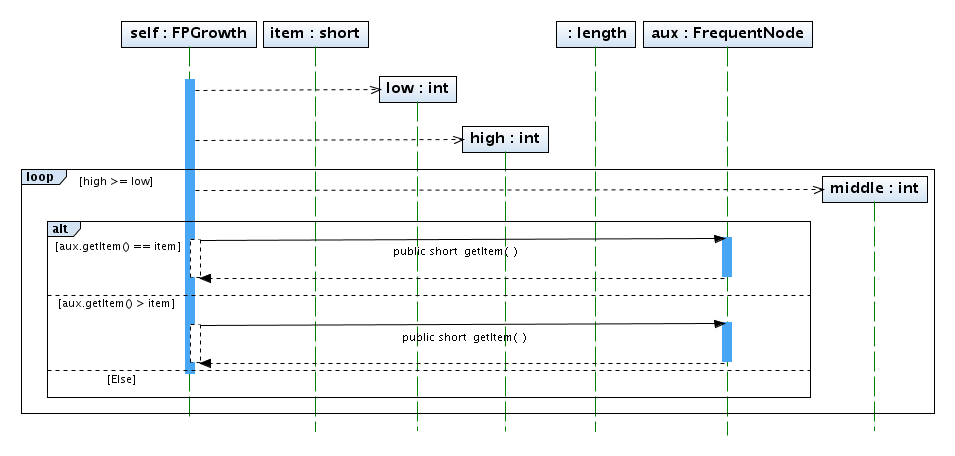
\includegraphics[width=1.2\textwidth]{imgsSecuencia/FPGrowth/findNode.png}
\caption{buildFrequentsNodes}
\end{figure}
\newpage
\begin{figure}
\centering
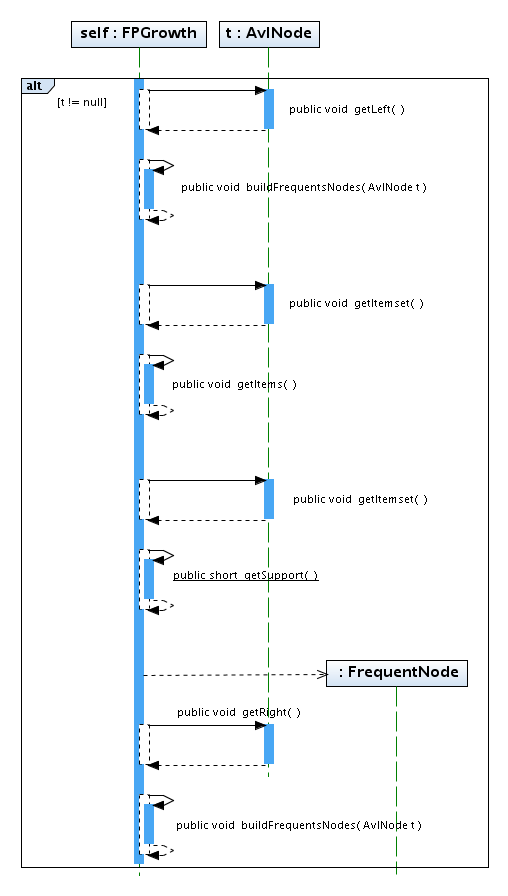
\includegraphics[width=0.7\textwidth]{imgsSecuencia/FPGrowth/buildFrequentsNodes.png}
\caption{findNode}
\end{figure}
\newpage
\begin{figure}
\centering
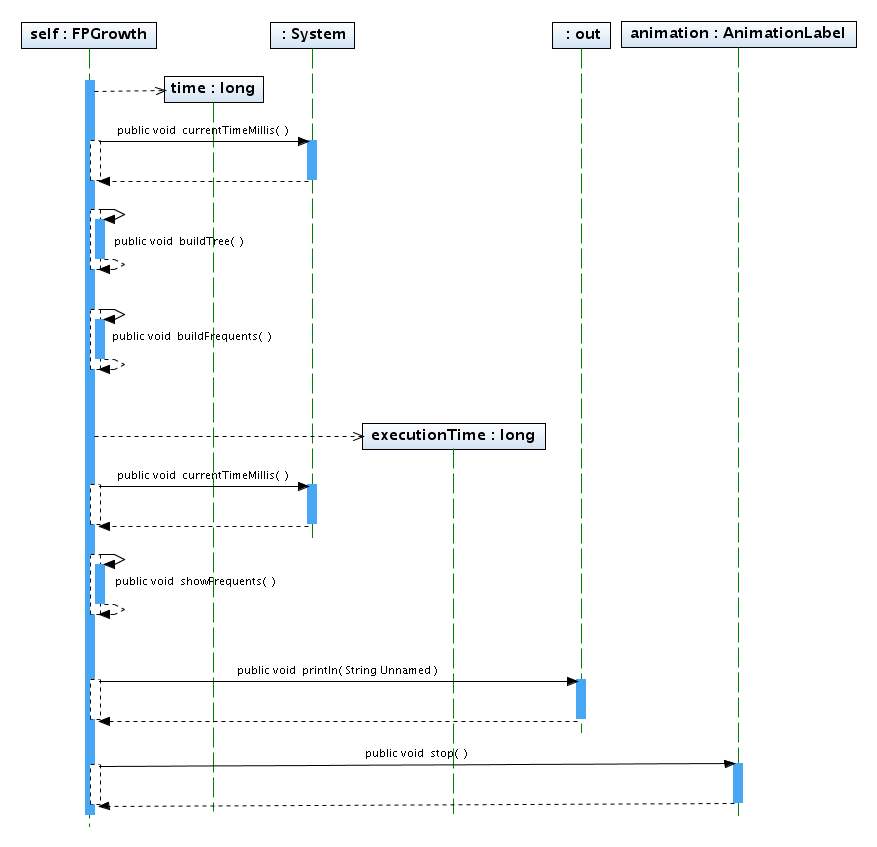
\includegraphics[width=1.2\textwidth]{imgsSecuencia/FPGrowth/run.png}
\caption{run}
\end{figure}
\newpage

%%%%%%%%%%%%%%%%%%%%%%%%% CLASE AVLTREE %%%%%%%%%%%%%%%%%%%%%%%%%%%%%%%%%%%%%%%%%%%%%%%%%
\begin{figure}
\subsubsection{Clase AvlTree}
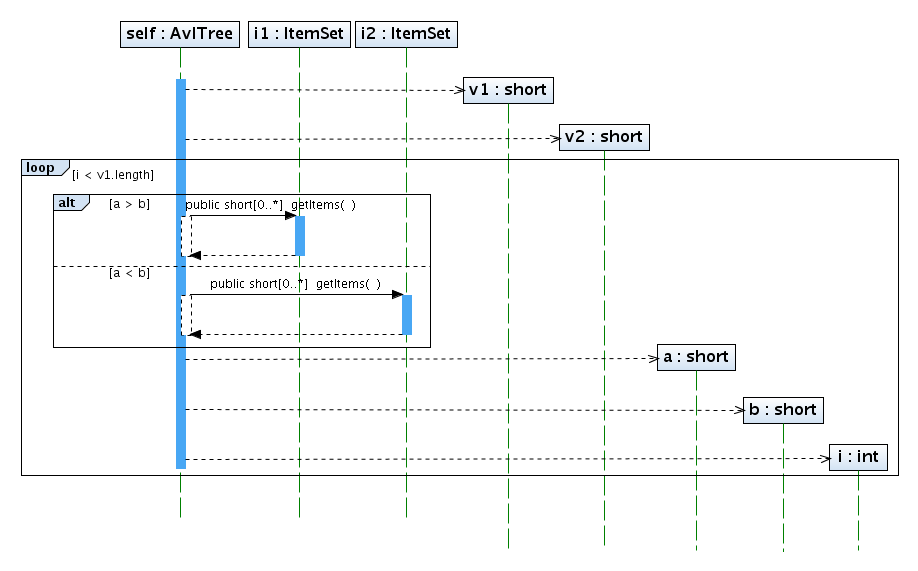
\includegraphics[width=1.2\textwidth]{imgsSecuencia/AvlTree/compareItemSet.png}
\caption{compareItemSet}
\end{figure}
\newpage

\begin{figure}
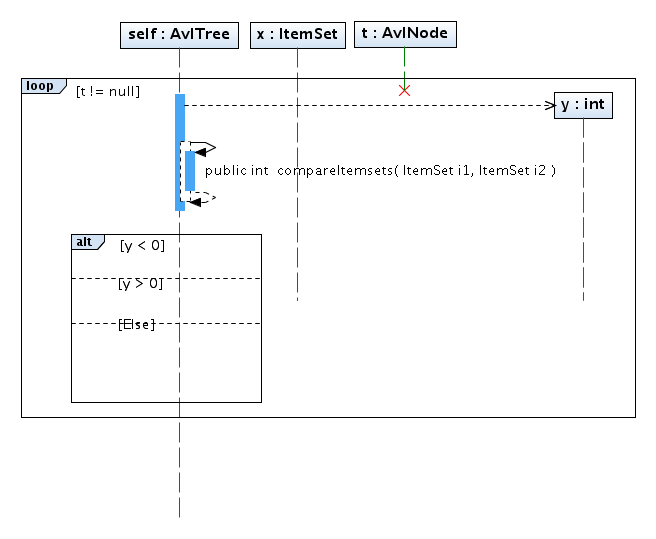
\includegraphics[width=1.2\textwidth]{imgsSecuencia/AvlTree/find.png}
\caption{find}
\end{figure}
\newpage


\begin{figure}
\centering
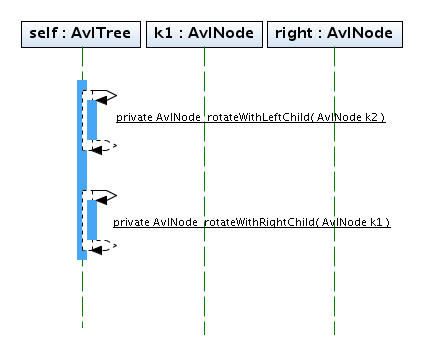
\includegraphics[width=0.8\textwidth]{imgsSecuencia/AvlTree/doubleWithRightChild.png}
\caption{doubleWithRightChild}
\end{figure}
\newpage


\begin{figure}
\centering
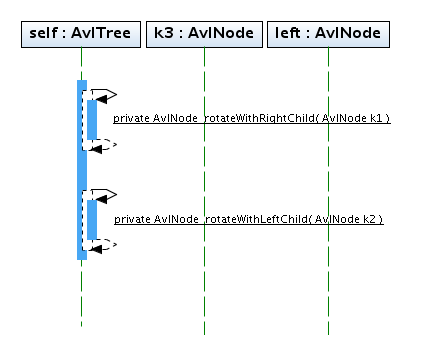
\includegraphics[width=0.8\textwidth]{imgsSecuencia/AvlTree/doubleWithLeftChild.png}
\caption{doubleWithLeftChild}
\end{figure}
\newpage

%%%%%%%%%%%%%%%%%%%%%%%%% CLASE TRANSACTION %%%%%%%%%%%%%%%%%%%%%%%%%%%%%%%%%%%%%%%%%%%%%%%%%

\begin{figure}
\subsubsection{Clase Transaction}
\centering
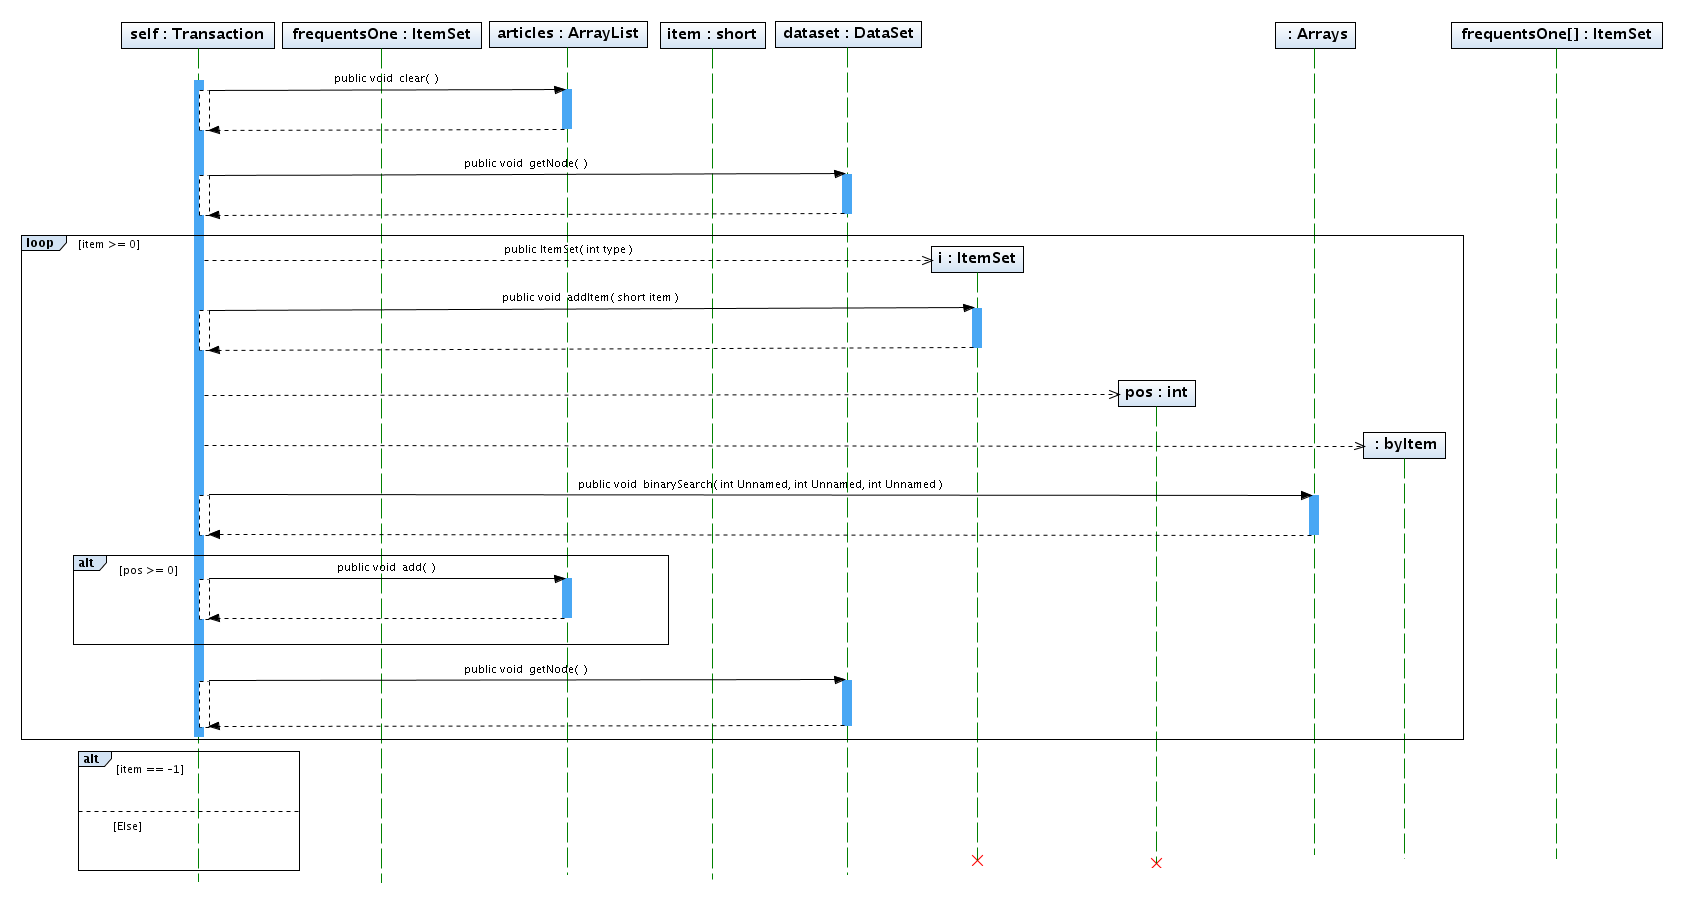
\includegraphics[angle=90, width=0.6\textwidth]{imgsSecuencia/Transaction/loadItemsets2.png}
\caption{loadItemset}
\end{figure}
\newpage

\begin{figure}
\centering
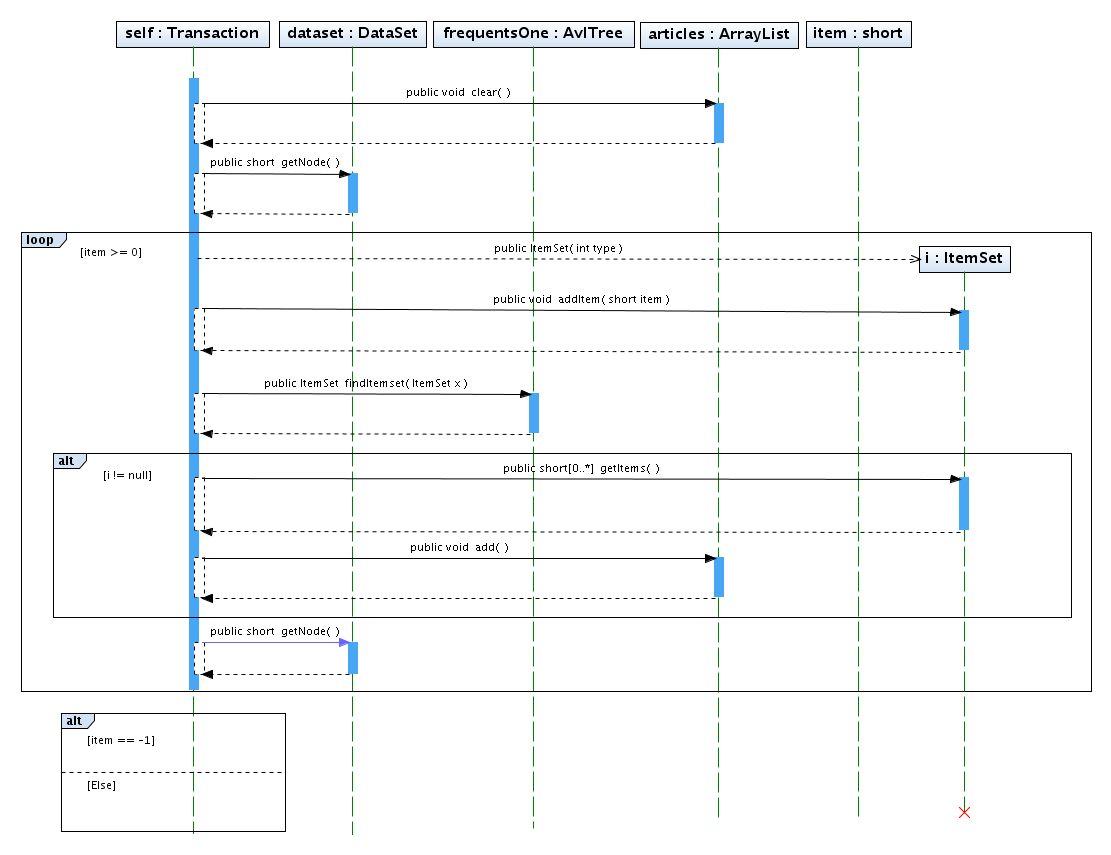
\includegraphics[angle=90, width=0.8\textwidth]{imgsSecuencia/Transaction/loadItemsets.png}
\caption{public-loadItemset}
\end{figure}
\newpage

\begin{figure}
\centering
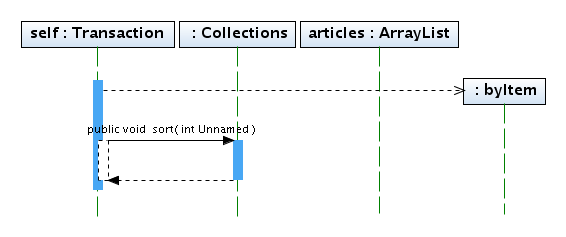
\includegraphics[width=1\textwidth]{imgsSecuencia/Transaction/sortByItem.png}
\caption{sortByItem}
\end{figure}
\newpage

\begin{figure}
\centering
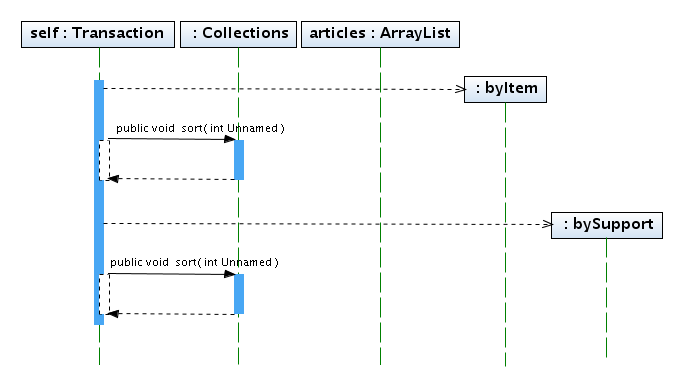
\includegraphics[width=1\textwidth]{imgsSecuencia/Transaction/sortBySupport.png}
\caption{sortBySupport}
\end{figure}
\newpage

%%%%%%%%%%%%%%%%%%%%%%%%% CLASE NODEF %%%%%%%%%%%%%%%%%%%%%%%%%%%%%%%%%%%%%%%%%%%%%%%%%

\begin{figure}
\subsubsection{Clase NodeF}
\centering
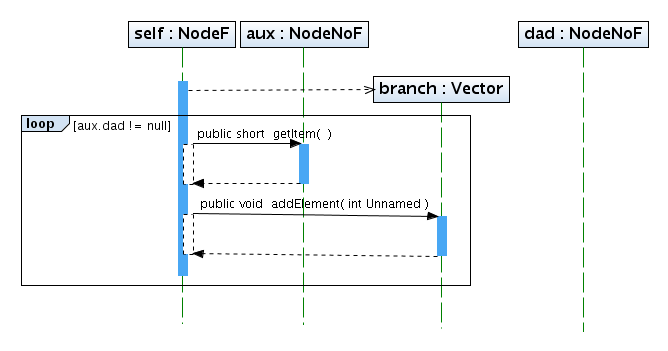
\includegraphics[width=1\textwidth]{imgsSecuencia/NodeF/getBranch.png}
\caption{getBranch}
\end{figure}
\newpage

\begin{figure}
\centering
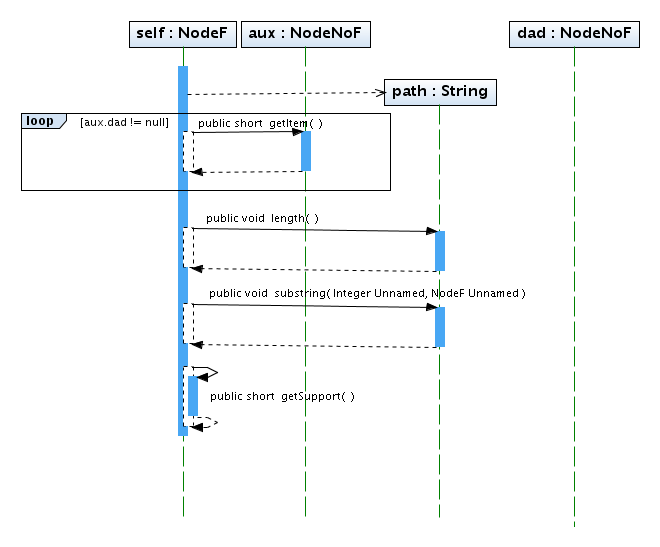
\includegraphics[width=1\textwidth]{imgsSecuencia/NodeF/getPath.png}
\caption{getPath}
\end{figure}
\newpage

%%%%%%%%%%%%%%%%%%%%%%%%% CLASE NODENOF  %%%%%%%%%%%%%%%%%%%%%%%%%%%%%%%%%%%%%%%%%%%%%%%%%

\begin{figure}
\subsubsection{Clase NodeNoF}
\centering
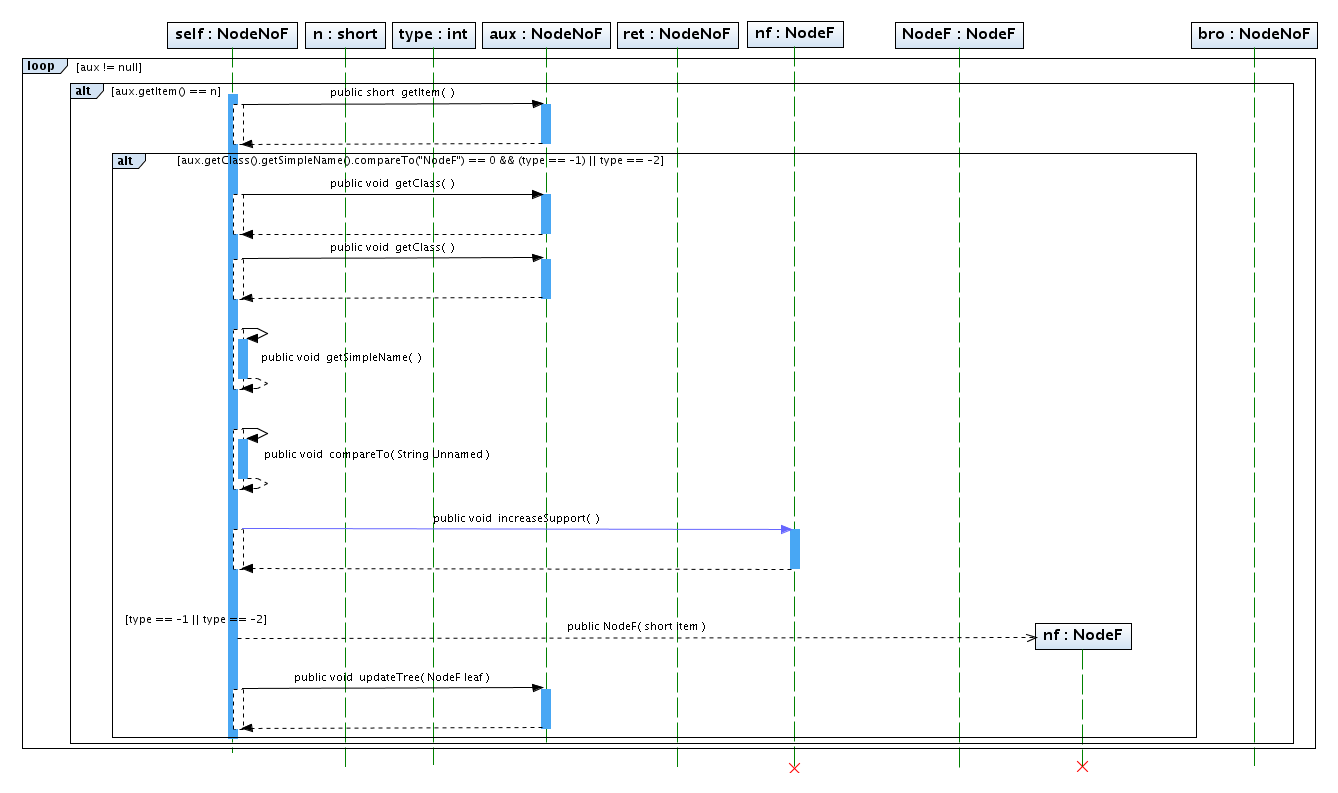
\includegraphics[angle=90, width=0.6\textwidth]{imgsSecuencia/NodeNoF/findBro.png}
\caption{findBro}
\end{figure}
\newpage

\begin{figure}
\centering
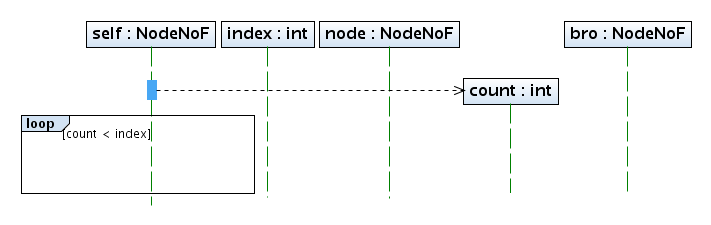
\includegraphics[width=1\textwidth]{imgsSecuencia/NodeNoF/getChild.png}
\caption{getChild}
\end{figure}
\newpage

\begin{figure}
\centering
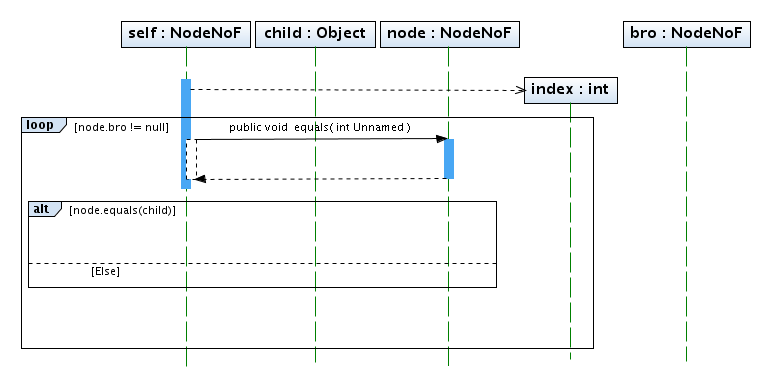
\includegraphics[width=1\textwidth]{imgsSecuencia/NodeNoF/getIndexOfChild.png}
\caption{getIndexOfChild}
\end{figure}
\newpage
% 
% \end{document}
